\documentclass[journal,twoside]{JoPhA}
\usepackage[utf8]{inputenc}
\usepackage{flushend}
\usepackage{graphicx}


\begin{document}

\title{VisualHFSM 5: recent improvements in programming robots with automata in JdeRobot}
 
\author{Samuel Rey and Jos\'e M. Ca\~nas
\IEEEcompsocitemizethanks{\IEEEcompsocthanksitem Samuel Rey and Jos\'e M. Ca\~nas are with Universidad Rey Juan Carlos\protect\\

E-mail: s.reye@alumnos.urjc.es, josemaria.plaza@urjc.es
%\IEEEcompsocthanksitem Vicente Matell\'an is with University of Rey Juan Carlos.
} % <-this % s
}

\markboth{Journal of Physical Agents,~Vol.~1, No.~1, July~2007}%
{Cazorla and Matellan : JoPhA Paper Demo}
\maketitle


\begin{abstract}
A visual programming tool, named VisualHFSM, has been improved in the JdeRobot robotics software framework. This tool provides Hierarchical Finite State Machines to program robot behaviors. The particular automata is designed visually, with nodes for the states, links for the transitions and specific source code on them. It automatically generates a C++ or a Python JdeRobot component that connects to the drivers and implements the automata. It uses multithreaded templates for that. Such component dynamically shows the current state of the automata while running. This tool speeds up the development time of robot behaviors, reducing the code that has to be created from scratch for new behaviors. VisualHFSM has been experimentally validated creating several autonomous behaviors for drones.
\end{abstract}


\begin{IEEEkeywords}
Visual languages, robot programming, automata
\end{IEEEkeywords}


\section{Introduction}

\IEEEPARstart{M}ost of the robot intelligence lies on its software. Its functionality resides in its programming, in the software that manages hardware resources like sensors and actuators. There is no universally standardized methodology to program robots. In the last few years the robotics community has begun to apply software engineering methodologies to its field, making more emphasis in code reuse, distributed software design, etc. Several robot programming frameworks that simplify the development of applications have emerged. 

These frameworks (1) provide a more or less portable hardware access layer (HAL); (2) offer a concrete software architecture to the applications; (3) include tools and libraries with already ready-to-use functionality and building blocks. Many of the emerged platforms are component oriented, such as ROS, Orca, Microsoft Robotics Studio, RoboComp, JdeRobot, etc..

In several frameworks, automata have been used for robotic software development. Finite State Machines (FSM) have been largely and succesfully employed in many fields and they can also be used in robotics to symbolize the robot behaviors, representing them in a compact and abstract form. With FSM the robot behavior is defined by a set of states, each of which performs a particular task. The system can then switch from one state to another through transitions, which are conditions of state change or stay depending on certain events or sensor conditions that may happen, both internal or external. FSMs provide one smart way to organize the control code and perception on-board a mobile robot. They have been explored in research and also incorporated in recent robotic frameworks with tools that let the programmer to focus on the behavior logic more than in implementation details. With these tools most of the code is then generated automatically from the abstract description of the FSM. This diminishes the chance of bugs, reduces the development time and allows the programming of complex behaviors in a robust way.

%paper goal
JdeRobot is the component oriented robot programming framework developed in Universidad Rey Juan Carlos. In this paper we present the new release of the VisualHFSM tool in JdeRobot, which supports the visual programming of robot behavior using hierarchical Finite State Machines. Now it can generate Python components, not only C++ ones. The generated components now show in a runtime GUI the active states in the hierarchical FSM. Its usability has been improved and support for drones has been included.

%paper organization
The reminder of this paper is organized as follows. In the second section we review related works on FSM tools in different frameworks. The third section presents the current visual programming tool emphasizing the improvements from the previous release. The fourth section describes two example applications generated with VisualHFSM for simulated and real drones. Finally, conclusions are summarized.

\section{Related works}

%Xait, videojuegos 
%Another  example  of  the  automaton  power  is  the  use for programming the intelligence of automatic players in videogames. This scenario is simpler than real robotic because much of the player perception is obtained looking up some videogame variable. 
Automata have been successfully used in videogame programming for generating the behavior of automatic players. For instance, Xait \footnote{http://www.xaitment.com} enterprise  commercializes  tools  that  facilitates automata programming to videogames developers, as its xaitControl (Figure \ref{fig:xaitcontrol}). This tool allows the programmer to  easily  develop  behaviors  with  hierarchical  finite  state machines. It has a main canvas in which the automaton is displayed, a tree view on the left shows the created structure and other panels show different information about auxiliary procedures, execution flow control, etc.. Another example is the successful best seller Halo 2 game of Bungie, where several automata were used to deploy more than one hundred different behaviors.

\begin{figure}[ht!]
\begin{center}
        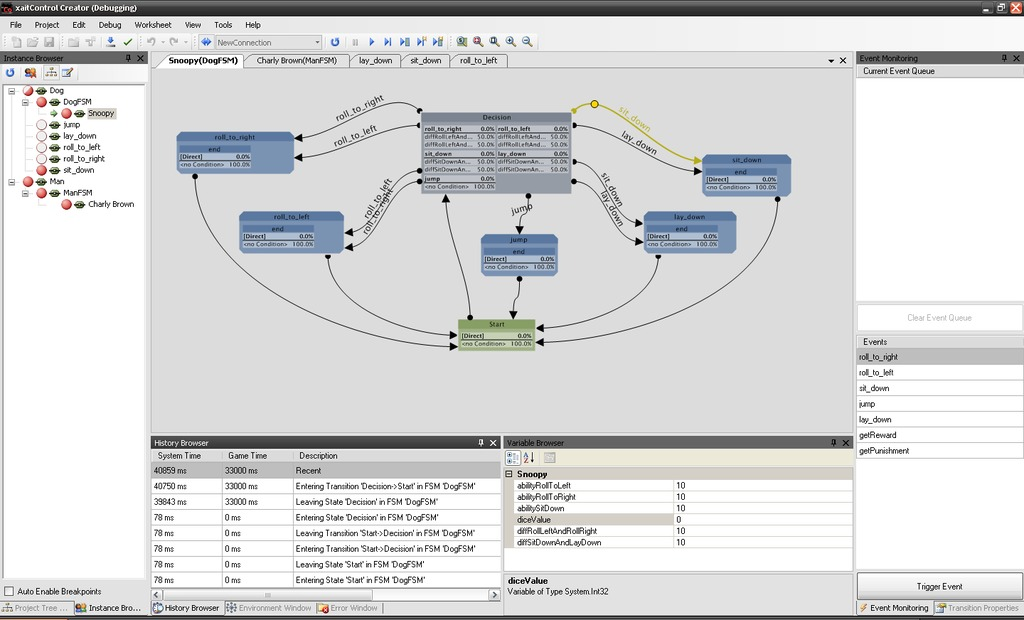
\includegraphics[width=8.5cm]{figs/xaitcontrol.jpg}
\end{center}
\caption{An instance of xaitControl}
\label{fig:xaitcontrol}
\end{figure}

%Smach
Regarding  finite  state  machines in robotics, in ROS framework there is SMACH \footnote{http://www.ros.org/wiki/smach} \cite{bohren2010,bohren2011}. This tool is a task-level architecture for rapidly creating complex robot behaviors. At its core, SMACH is a ROS-independent Python library to build hierarchical finite state machines. To develop a hierarchical finite state machine you have to write the code needed to create and describe each state and transition, it is not a visual tool. The package also comes with the SMACH-viewer (Figure \ref{fig:smach}), a tool that shows the developed finite state machine at runtime. In that tool, we can see either a graph or a tree view of the current automaton, but not both at the same time. It also shows every state and transition, as well as the active state and a debug window where we can see data of the active state.

\begin{figure}[ht!]
\begin{center}
        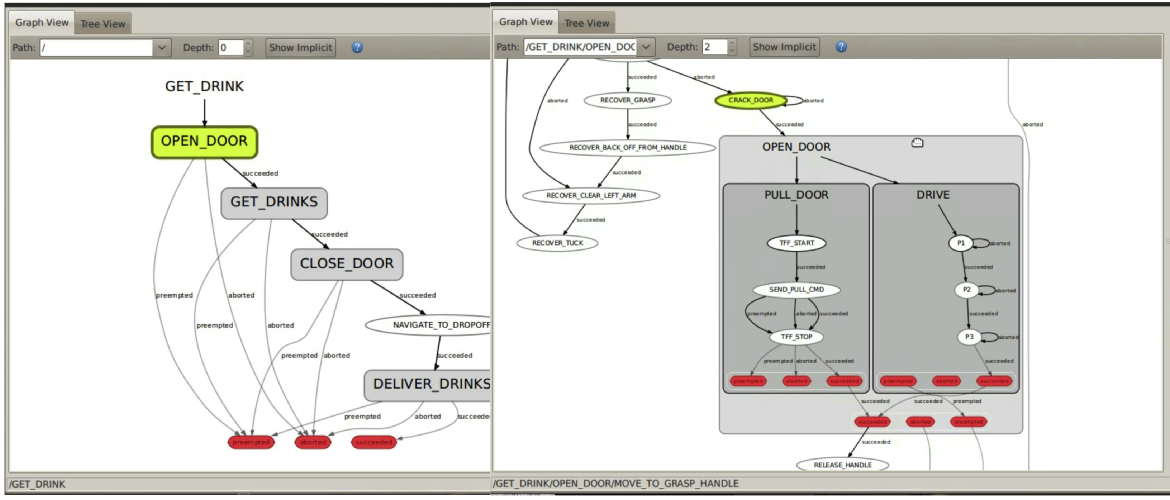
\includegraphics[width=8.5cm]{figs/smach-viewer.png}
\end{center}
\caption{An instance of SMACH-viewer}
\label{fig:smach}
\end{figure}

%MissionLab
One of the most powerful frameworks that use HFSM in robotics is MissionLab, developed in Georgia Tech by the professor R. Arkin. This environment includes a graphical editor of  configurations  (CfgEdit) \cite{mackenzie1998} as a tool, similar to  automaton,  that  allows  to  specify  missions  with  its states, transitions, etcetera. It allows to generate applications following the AuRA architecture, developed by the same group. In order to represent the automaton they developed their own language, the Configuration Description Language. A more recent example of FSM is the automaton editor inside the component-oriented platform RoboComp, from Universidad de Extremadura. For instance, in \cite{cintas2011}, they used it to program the behavior of a forklift. Another sample is the behaviors graphical editor Gostai Studio \cite{gostai2012}, inside the Urbi platform. This graphical editor generates urbiscript code as its output, includes time-execution visualization of the state of the automaton, allows to stop and continue the execution of the generated automaton and offers the possibility of creating hierarchical finite state machines.

%XABSL
In the RoboCup scenario finite state machines are frequently used to generate behaviors for the standard SPL league humanoid robots. Several teams use the tool and language XABSL \cite{lotzsch2004,risler2009} to specify behaviors, around the influential German team B-Human. In addition, the TeamChaos team \cite{herrero2006} used an HFSM tool to handle hierarchical finite state machines for its architecture ThinkingCap, allowing even behavior hot-edition in each state. In SPIteam a tool named Vicode is used to generate finite state machines for BICA architecture.

%refs de Joaquín y sus redes de Petri


\section{Improvements in VisualHFSM 5}
%general presentation
VisualHFSM \cite{borja2013} is a tool created for the programming of robot behaviors using hierarchical finite states machines. It generates as output a component in JdeRobot framework that implements the robot behavior. It represents the robot’s behaviour graphically on a canvas composed of states and transitions. 

The source text code to be executed in each state or transition must be introduced. This tool decreases the development time for new applications, providing the developer with a higher level of abstraction. It also increases the quality of these applications, automatically generating most of the code using a clean and well organized template. The tool allows the engineer to focus on specific parts of her application, writing only the actual code that will be executed by the automaton and the conditions that will make the robot to go from one state to another. The final result is a more robust code and less prone to failure. 

% explained before, VisualHFSM is a flexible tool that allows its users programming code for several different type of robots, saving time by focusing only in programming the code that actually depends on the automata behaviour, and auto-generating the complete code of the automata by completing a template, achieving in this way a robust and well organized code minimizing the effort of the developer.

%visualHFSM parts
VisualHFSM is divided in two parts: a \textit{graphical editor} and the \textit{automatic code generator}. The graphical editor displays the main window where the automaton structure is created. It also contains internal structures and saves all the data into an XML file. %The aspect of this graphical editor in VisualHFSM is shown in the figure \ref{fig:editor}. 
The automatic code generator reads that XML file 
%that was created and saved using the graphical editor, 
and delivers the source code of a JdeRobot component implementing the HFSM. It also generates a configuration file for it. The compilation can be launched from the graphical editor or outside.

% created from the parameters passed through the graphical interface and a CMake file for compiling the automata. The compiling is also done using the main window of the graphical editor, and it will leave an executable file in the path where the XML has been saved.

%It has a graphical editor and an automatic code generator. The graphical editor still displays the main window where all functionality is located to create the automata, and all of this functionality that compose the automata is saved inside a XML file. The main changes are related to the automatic code generator, as explained before, it generates C++ and python code.  This will be explained in more detailed in the following sub chapters. 

The previous release of VisualHFSM had several shortcomings and limitations. Most of them have been addressed in the fifth release and are described next.

\subsection{Better usability in the graphical editor}

The graphical editor allows the developer to see, edit and add states and transitions in a clear and simple way. The component is represented by a finite state machine in a canvas, where all elements are visualized. It allows to manipulate states (create, remove, move, rename...) and to define the behavior that will be executed in them. It is also possible to set the conditions for regulating the transitions between states, and the code that will be executed when the transitions occur.

\begin{figure}[ht!]
\begin{center}
        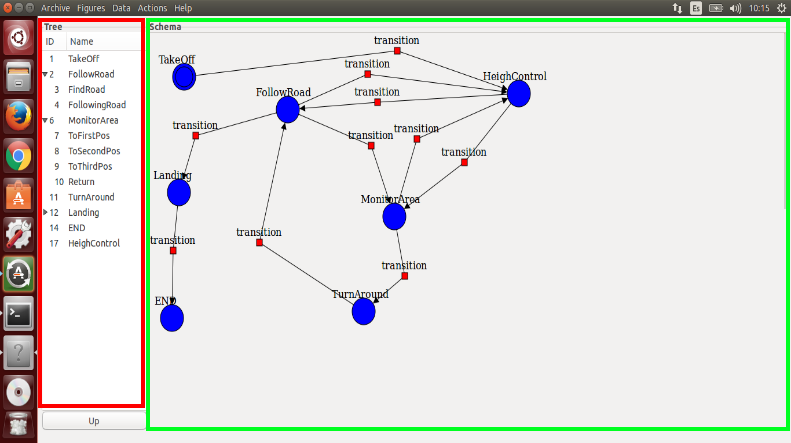
\includegraphics[width=8.5cm]{figs/editorColor.png}
\end{center}
\caption{Graphical editor of VisualHFSM 5.0}
\label{fig:editor}
\end{figure}

As shown in the Figure \ref{fig:editor}, the GUI in VisualHFSM 5.0 is now divided into two parts: the \texttt{Tree View} at the left and the \texttt{Scheme View} at the right. The buttons part of Figure \ref{fig:editor-old}, present in previous releases, is now placed in the \texttt{menu bar}, so the space of the window for creating the automaton is bigger and more comfortable. Another usability improvement is that now the canvas, the \texttt{Tree View} and all of the popup elements are scrollable.

\begin{figure}[ht!]
\begin{center}
        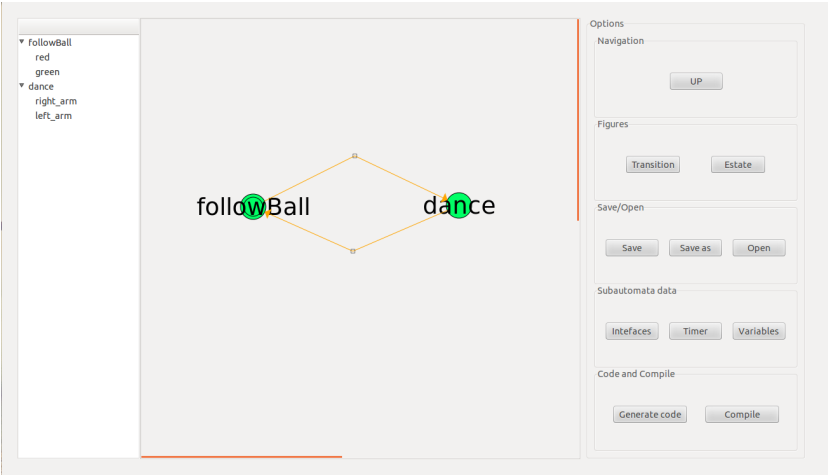
\includegraphics[width=8.5cm]{figs/editor-old.png}
\end{center}
\caption{Graphical editor of previous version of VisualHFSM}
\label{fig:editor-old}
\end{figure}

In the \texttt{Tree View} (red border area in Figure \ref{fig:editor}) the whole automata is text represented in the hierarchical mode with two columns for identifying the states: one for the ID and other for the name given to this state. It has now the option of collapsing or expanding the children of some state, so the developer can choose to see all the levels at the same time or focus on some specific levels by collapsing the rest. The children and levels of the hierarchy are represented under their fathers by using different tabulations. It allows a simple and intuitive navigation through the automaton, double clicking in one state for representing the subautomaton that it contains.

In the \texttt{Schema View} (green border area in Figure \ref{fig:editor}) the automata is graphically drawn, showing the name of each state or transition. States are represented as blue circles and for each subautomata it also marks with a double circle the state which must be active at the beginning. For each state, the user can rename it; edit it, allowing to change the code of the selected state; mark it as the initial state of its subautomata; copy it, allowing to paste the selected state into another or the same subautomata; and delete it. Any state can be connected to another by an unlimited number of transitions or to itself by auto-transitions. Transitions are represented as arrows that go from the origin state to the destiny, with a red square in the middle for applying them different actions, as move them, rename them, editing its condition, adding them code and delete them. The condition added by editing a transition is the condition that must happen for the transition to occur. The Schema View also allows to graphically navigate through the automata double clicking in the desired state or in the \texttt{Up} button. %, just under the \texttt{Tree View}.

In the \texttt{menu bar}, menus are structured in five groups: Archive, Figures, Data, Actions and Help. The Archive menu allows to create new projects, open existing ones, saving the current project or exit VisualHFSM. Figures menu contains two buttons, for adding new states or transitions. Data menu has Timer, for choosing the frequency of the iterations, and Variables, for adding variables and functions that the developer may need for better organizing and structuring its code, giving more flexibility to the tool. Last, the Actions menu allows to add additional libraries that the automata code may need, edit the parameters for the “Config file” that will be auto-generated with the code, generate C++ or Python code and compile the C++ code by using the CMake file generated with the code.

\subsection{Runtime GUI in the generated C++ component}

For running the automata, the XML file is parsed and a new JdeRobot component in C++ is generated. Such C++ component implements the automaton and is generated using a carefully designed \textit{C++ template}. Each subautomaton is implemented as a single thread, so the full automata is a collection of concurrent threads which interact among them, sleep, are resumed, etc. as some states of the automaton are activated or deactivated. More details of this template can be found in \cite{borja2013}.

The new VisualHFSM 5 includes some code to graphically show the (hierarchical) automaton state at runtime. If the user wants it, the generated JdeRobot component displays a runtime GUI that shows which states are active or not while running. This is very convenient for debugging. %The developer may check in a natural way whether the robot’s behavior is the same as expected, or whether the automata transits from one state to the intended one.

\begin{figure}[ht!]
\begin{center}
        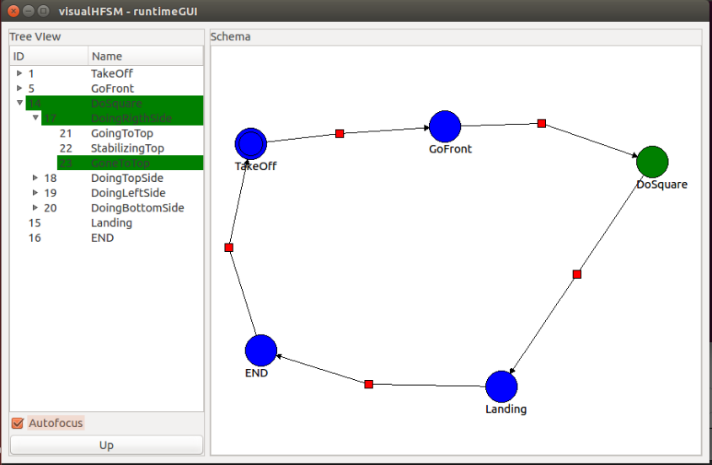
\includegraphics[width=8.5cm]{figs/runtime.png}
\end{center}
\caption{Runtime GUI in C++ component using the Autofocus feature}
\label{fig:runtime}
\end{figure}

%use
Figure \ref{fig:runtime} shows one runtime GUI similar to the graphical editor. %It also has two sections, the Tree View and the Schema View, but instead of allowing editing the automata, it represents the states that the automata is currently executing. 
%For indicating which states are active, t
The current active states are displayed with green background color in the TreeView, in all levels of the hierarchy including the root. The user may expand or collapse the different hierarchical levels at will. In addition, a check box named “Autofocus” has been added. When selecting it, the Tree View will automatically expand and collapse itself for showing the active states and the rest of the automaton will be collapsed, as shown in Figure \ref{fig:runtime}. In the Schema View of this runtime GUI, the active nodes are presented in green and the others in blue. When a transition takes place, the old active state is painted in blue in the Schema View and with white background in the Tree View, and the new active state is painted in green and with green background in the Tree View.

This runtime GUI feature is off by default, because the graphical window is useful only for debugging. In normal robot operation, once its behavior programming has been refined, there is no need to spend computational resources in this additional GUI. Nevertheless, it is very useful in the developing process. Enabling this feature is as easy as executing the component with the flag \texttt{--displaygui=true}. 
%If the component is executed by default, the runtime GUI will not be created, so it will have no impact in the robot’s performance.

%implementation
The runtime GUI has been implemented as an additional thread and a new library called \texttt{automatagui}. %This library includes all the functionality for using the runtime GUI. %At run time the component does not require the XML file created by the graphical editor. 
When the code or the C++ component is being generated, a C++ function is written for constructing a list containing all subautomatas with its states and transitions. An object of the class \texttt{AutomataGui} is created and inserted in the component. The component will use at runtime that object for dinamically showing the automaton. %That object will also be responsible for changing the color of the states when the active state changes. 
% To avoid race conditions on doing so, when a state is going to be active the thread responsible of executing this subautomata code sends a notification to the GUI thread using a Dispatcher object, and the \texttt{AutomataGui} object will do the rest. 

\subsection{Generation of Python component with its runtime GUI}

In the new release of VisualHFSM, the robot behavior may be programmed in Python too. Adding support for this language, VisualHFSM increases its flexibility and the component does not requires to be compiled. The code inserted for the states and transitions in the graphical editor must be in Python and a new template in Python has been developed to generate the component's final code. 

The code is now organized following an object oriented model. There will be the main class \texttt{Automata}, which will contain all the information related to the automaton. This approach makes easier the communication between different subautomata, or different threads, by using elements of the \texttt{Automata} class instead of global variables. It also provides a threading lock, in case some code is sensitive to race conditions and it allows to create inner classes, in addition to more functions or variables that could be needed. The additional features will also be created inside the \texttt{Automata} class. This implementation provides more robust, better organized and cleaner code. In addition, as Python do not need to compile, it is faster to make any change on the program. The Python code is generated as an executable. %, so it can be called in the same way as the C++ executable.

For unfolding the runtime GUI the Python component must be launched with the \texttt{--displaygui=true} parameter too. It has been programmed using the PyQt4  graphic library in Python. The way of communicating that the color of a state needs to change is simpler than in C++. It is implemented by the GUI thread again to avoid race conditions, but this time the notification is done using a handler. The thread that is going to change its active node will emit a signal with the node name, which will be handled by a handler in the GUI thread. 
%After the notification, the processing is the same as it was in the C++ component. 

In this release it is possible to create several runtime GUI windows (one for one subautomaton in detail), if convenient. To activate a new window the user only has to right click over one state of the desired subautomaton and then select “Open Subautomaton”. Figure \ref{fig:runtime-hierarchy} shows several subwindows.

\begin{figure}[ht!]
\begin{center}
        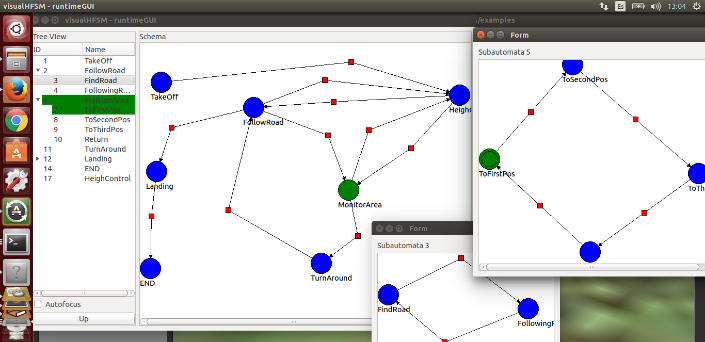
\includegraphics[width=8.5cm]{figs/runtime-hierarchy.png}
\end{center}
\caption{State diagram of the monitor-an-area application shows three subautomatas at the same time}
\label{fig:runtime-hierarchy}
\end{figure}

\subsection{Support for drones}

Several real robots as Pioneer from ActivMedia, Kobuki (Turtlebot) from Yujin Robot, Nao from Aldebaran and their counterparts in Gazebo simulator were supported in previous releases of VisualHFSM. In the new release support for ArDrone-1 and ArDrone-2 from Parrot and simulated drones in Gazebo has been included. Their corresponding JdeRobot interfaces and their local data structures are now available for use from the code of the states and transitions.

\subsection{Shutdown}

Another feature added in this release, both in Python and in C++, is the \texttt{Shutdown} function. This function ends the loop of all the subautomata by setting the correspondent variables to false, so the code will reach the end and finish, in contrast with previous releases of VisualHFSM, where the execution never ended unless the process was manually interrupted from the terminal.

\section{Experiments}

In order to validate the new features introduced with this version of VisualHFSM, we have performed two different experiments, both of them using a simulated ArDrone robot. The experiments are two robot applications developed using visualHFSM: monitor-an-area application and follow-colored-objects applications. Both of them are written using the Python code generator of VisualHFSM.


\subsection{Monitor-an-Area application}
%application description
For this first application, we have used a Gazebo scenario with a road, and some victims of a car accident laying in the ground around the location were the accident has occured. This simulated scenario is an example of an application where drones could be useful: go fast to the accident place and check with its camera the status of the victims, for the emergency service to give a better, faster and more accurate response. 

%HFSM-based solution
We identified several states to unfold different behaviors of the robot in this example. Their combination into a HFSM fulfils the whole application. First, the drone has to take off. When it has reached the desired height, it goes to the next state \texttt{following-the-road}. Figure \ref{fig:followingRoad} shows the ArDrone following the road in that state. This state has a child subautomaton, for following it and considering other aspects at the same time. For instance, if the drone lost the road, this child subautomaton tooks control to search and recovers the road again. After finding it, it returns to the state of following the road. 

\begin{figure}[ht!]
\begin{center}
        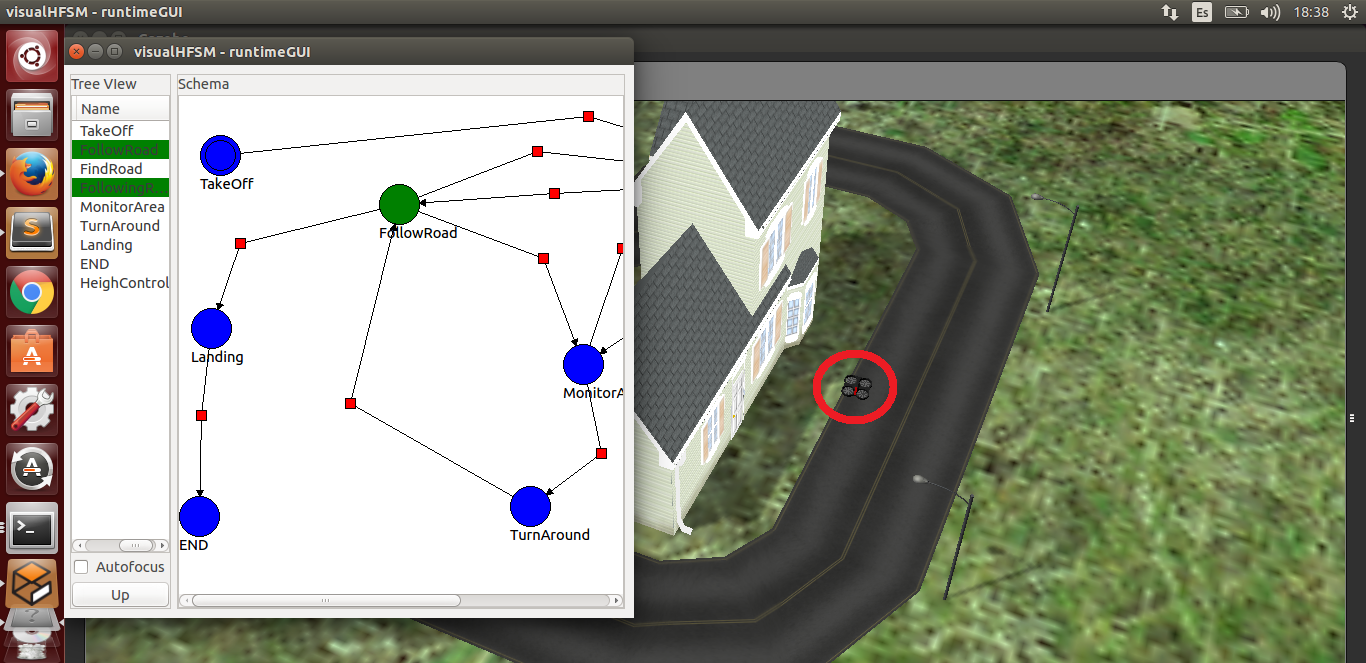
\includegraphics[width=8.5cm]{figs/followingRoad.png}
\end{center}
\caption{ArDrone following the road}
\label{fig:followingRoad}
\end{figure}

It will keep in the \texttt{following-the-road} state until it gets to the point where the accident has happened. Then, it switches to the \texttt{monitor-area} state, which is responsible of looking for and locate the victims, as shown in Figure \ref{fig:watchPerson}, where the drone has found a victim. This state has a child subautomaton for specifying phases of this activity in a simpler and more understandable way. 
When it has finished searching in the area, the drone will come back to the point of the road where it started to search for victims, it will turn around, and again it will go to the \texttt{following-the-road} state, following it until it reaches the point where the drone took off, and then lands there. 

During all the execution, the height of the drone has been watched. If it went too hight or too low, the automaton would have switched to another state until it reaches the desired height. The state diagram of this behavior is shown in the Figure \ref{fig:runtime-hierarchy}, where we can see the root subautomaton, and those of \texttt{following-the-road} and  \texttt{monitor-area} states. 

\begin{figure}[ht!]
\begin{center}
        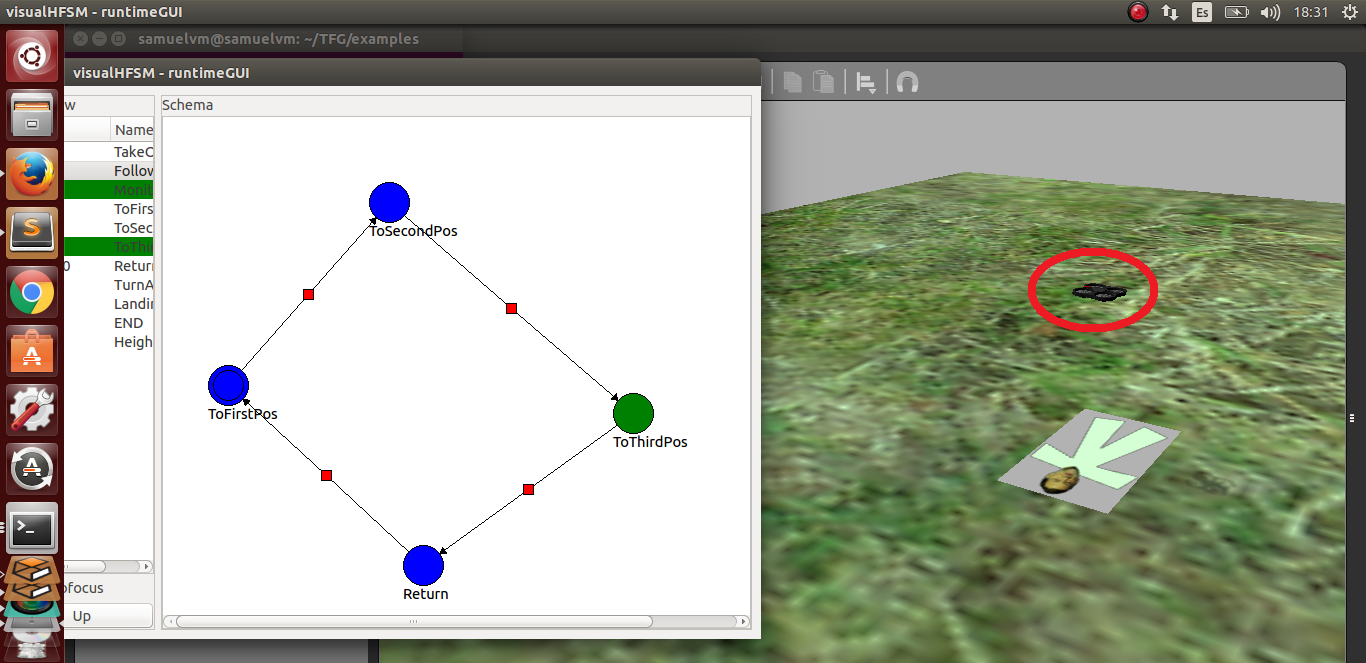
\includegraphics[width=8.5cm]{figs/watchPerson.png}
\end{center}
\caption{ArDrone recording the location of a car accident's victim with its camera}
\label{fig:watchPerson} 
\end{figure}



\subsection{Follow-colored-objects application}

%application description
The motivation for this application is to use visualHFSM with a real robot, an ArDrone2 from Parrot. In this experiment there are several different colored moving objects, and the ArDrone must follow them using its ventral camera following a sequence. First, it will follow the green object until it finds something blue, then it will start following this new blue object until it finds a green object again. Finally, it will follow such green object until it finds a red one, which it will follow until the application finishes.

\begin{figure}[ht!]
\begin{center}
        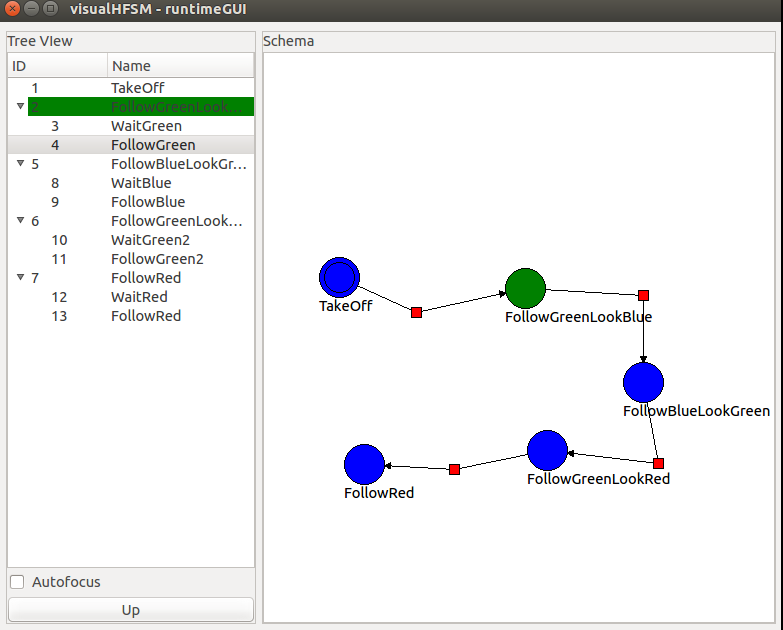
\includegraphics[width=8.5cm]{figs/colorsStatesGUI.png}
\end{center}
\caption{State diagram of the follow-colored-objects application from its runtime GUI}
\label{fig:statesColors}
\end{figure}

This kind of behaviour perfectly matches a HFSM, as each of the four stages of following an object while looking for another can be modelled with states and transitions. The state diagram is shown in Figure \ref{fig:statesColors} when the Robot is following the green object and looking for a blue object. The whole automaton is expanded on the Tree View.

%implementation
As it is shown, the drone starts in the \texttt{take-off} state. When the desired height is reached, the drone will go to the state \texttt{FollowGreen-LookForBlue}. There it will be filtering two colours: green and blue. It will be following the green object until it detects a blue contour, and then it will change to \texttt{FollowBlue-LookForGreen} state. Then, to avoid the drone immediately detecting the green object that it has been following in the previous state, it will wait a blanking interval. During this interval it will only follow the blue. When such interval is over, in case of finding a green contour it will change to \texttt{FollowGreen-LookForRed} state. This state works like the other two, and when the drone finds the red object it will change to \texttt{FollowRed} state until the program finishes. Figure \ref{fig:followingRed} shows the real drone following this last red object.

% \begin{figure}[ht!]
% \begin{center}
%         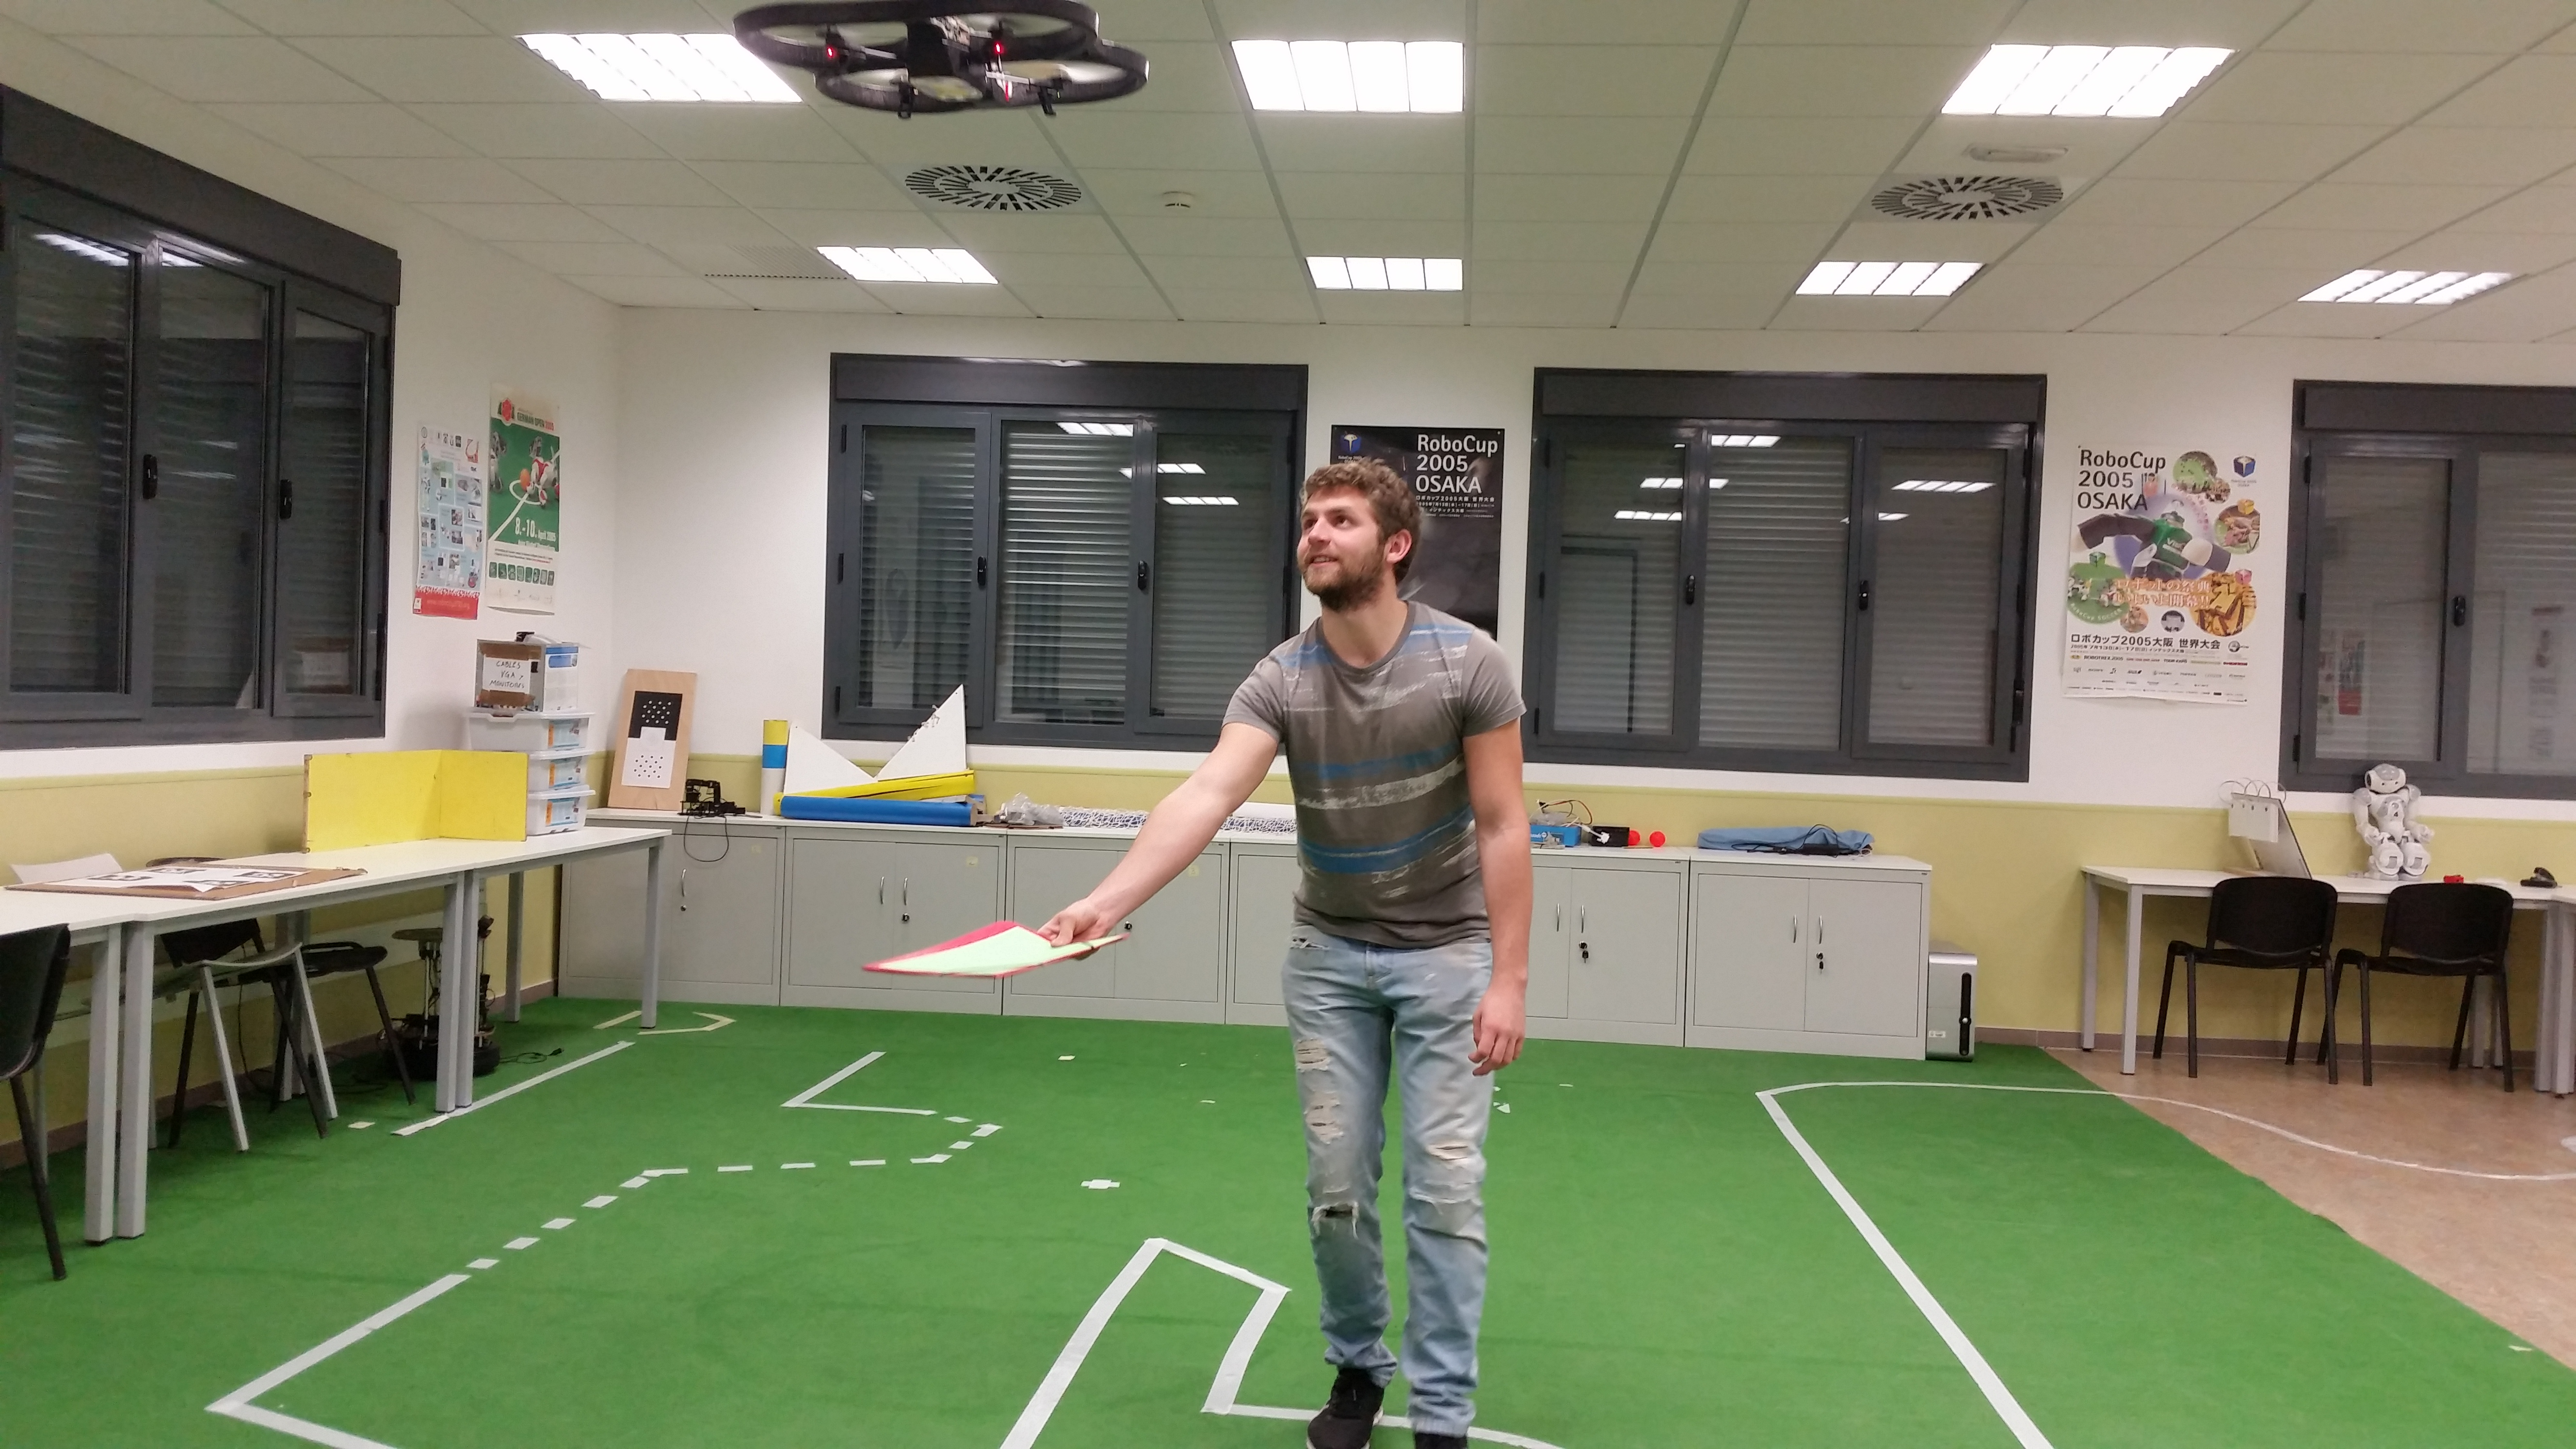
\includegraphics[width=8.5cm]{figs/followingGreen.jpg}
% \end{center}
% \caption{ArDrone robot following the green colour inside the state FollowGreen-LookForBlue.}
% \label{fig:followingGreen}
% \end{figure}

\begin{figure}[ht!]
\begin{center}
        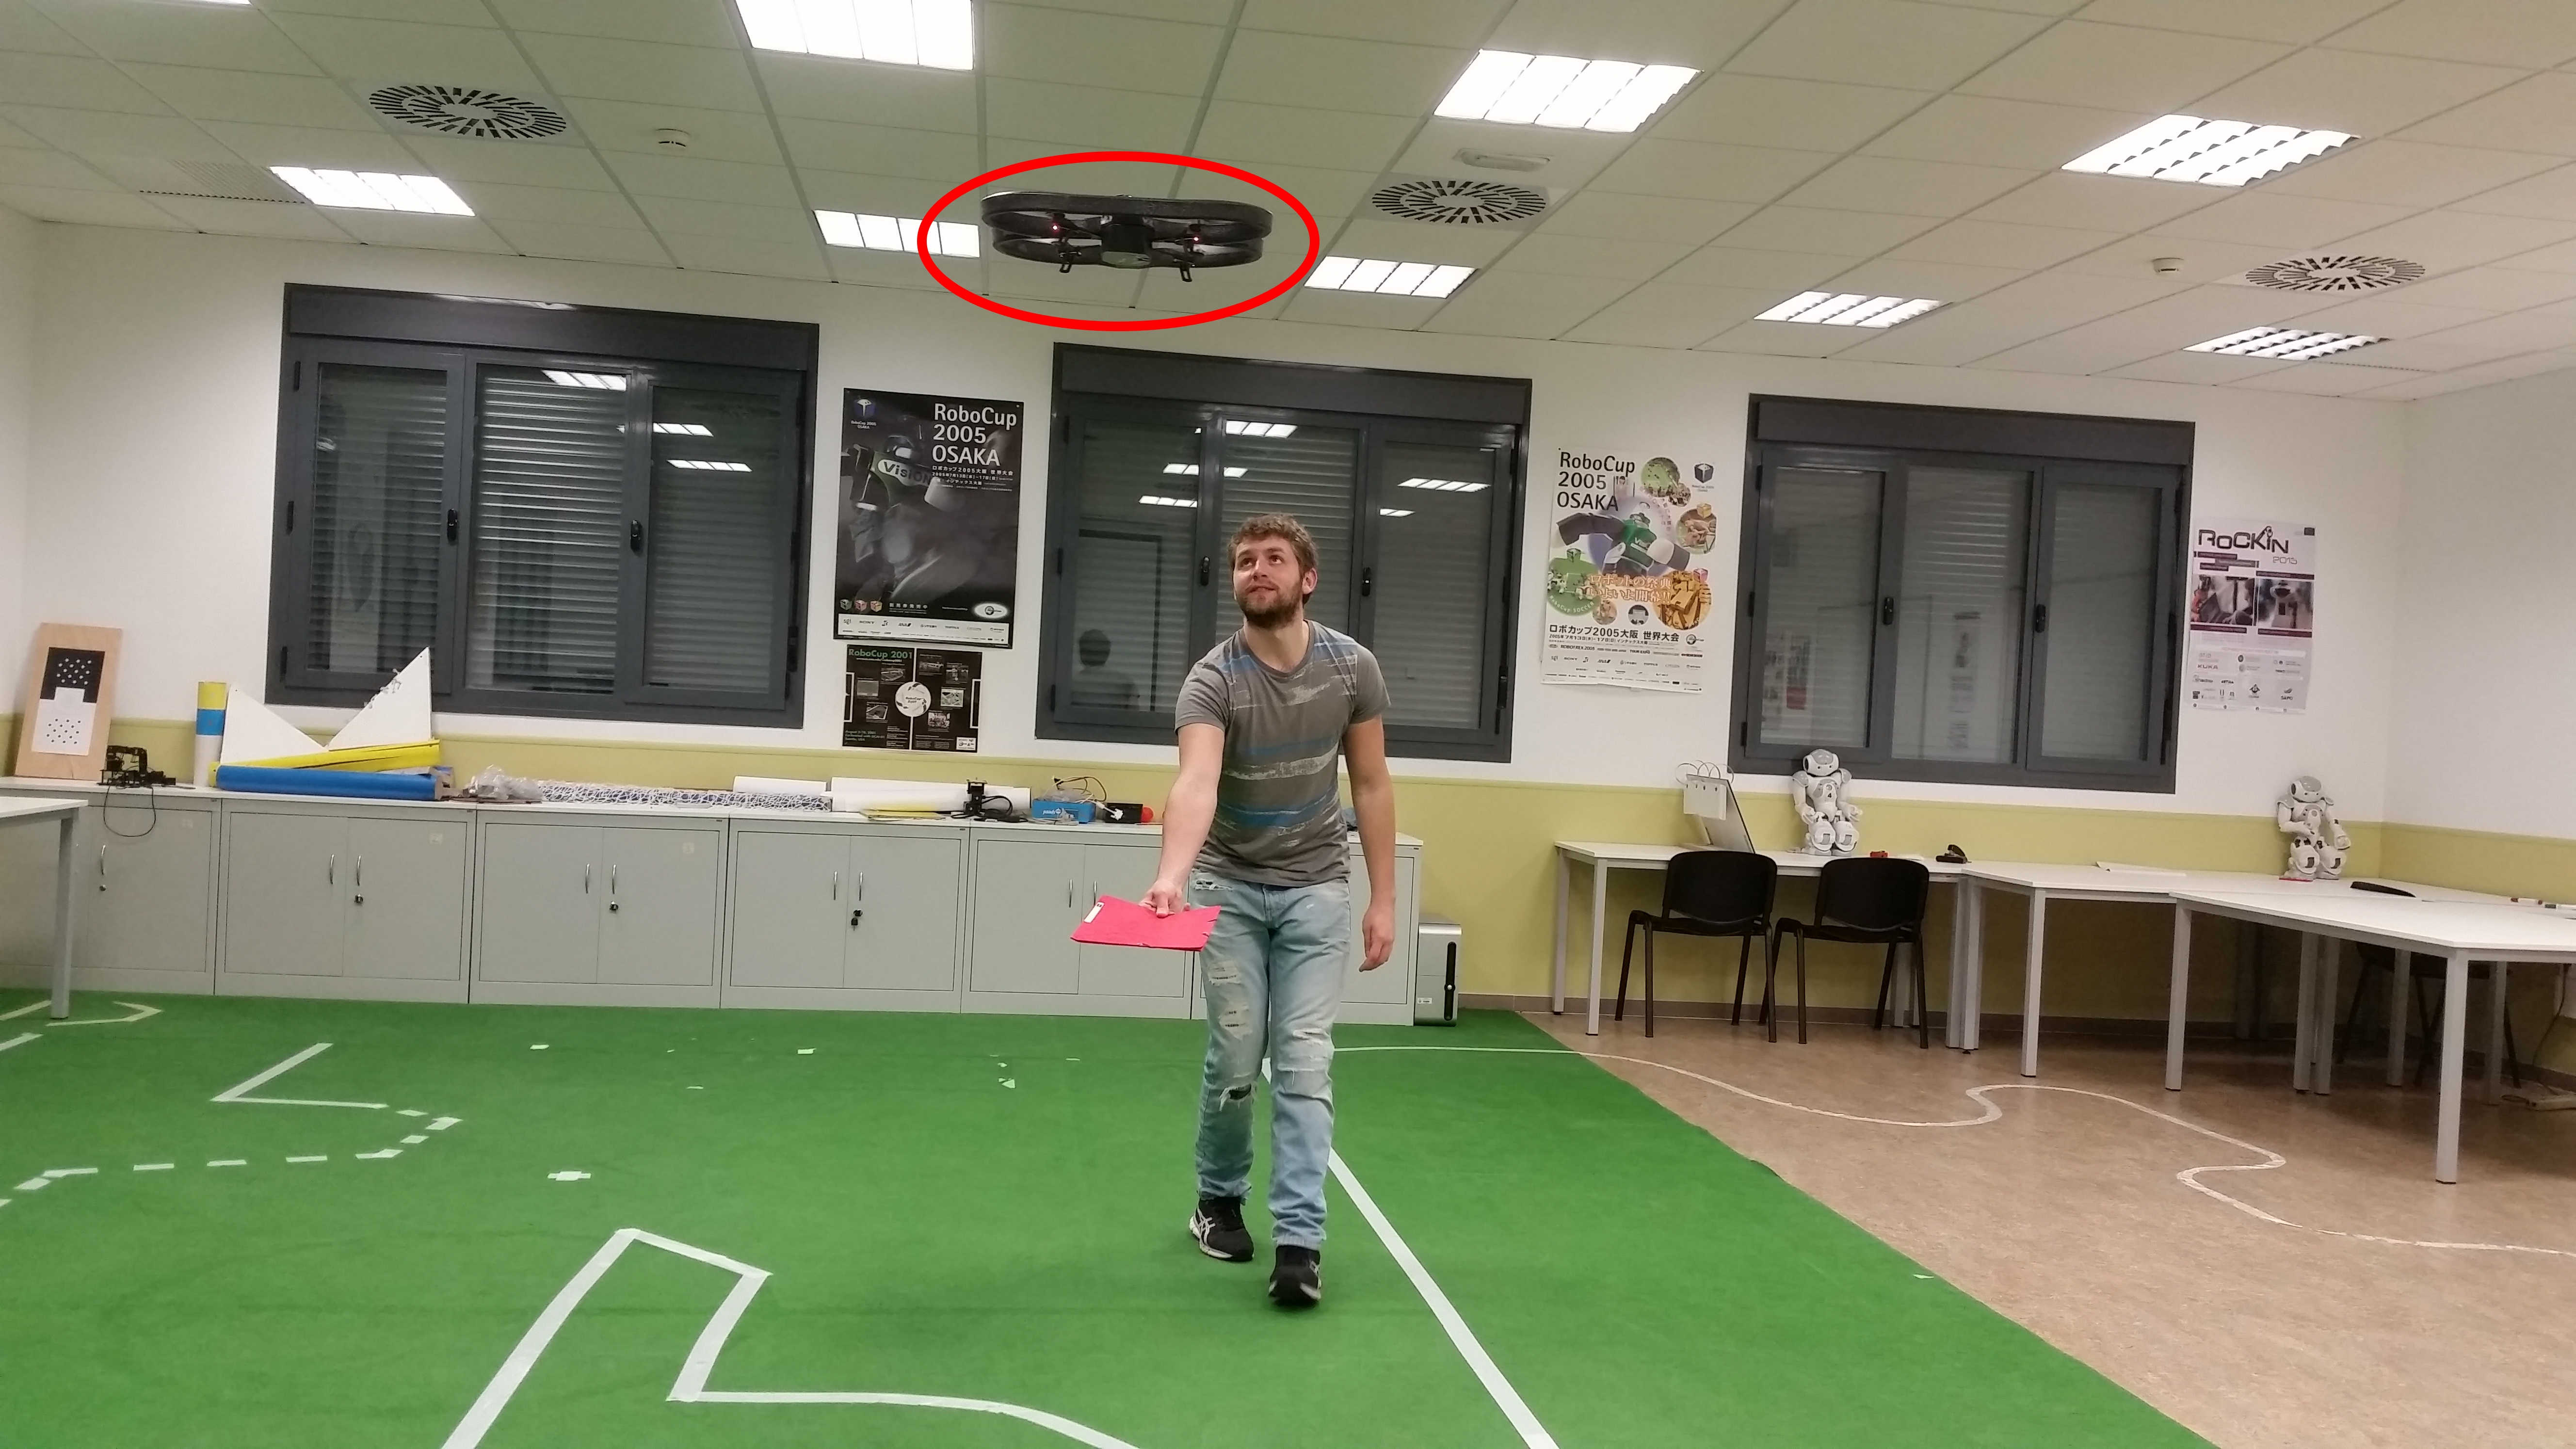
\includegraphics[width=8.5cm]{figs/followingRed.jpg}
\end{center}
\caption{ArDrone robot following a red object in the \texttt{FollowRed} state.}
\label{fig:followingRed}
\end{figure}

All the color following states are implemented with a child subautomaton. The father is in charge of detecting the colors and decides if it should continue in the current state or go to the next, while the children is responsible for following the color. We have followed this approach because the laboratory where the experiments have been performed is small, and so, when the drone loses the color it is following, it should stop. In other scenarios like open spaces it would be more convenient that when the drone loses the object, it would start a looking for manouver. With this approach it would be easier to have a new child subautomaton performing such manouver.

This experiment has been performed both using Gazebo simulator and real robots. In Gazebo it works perfectly, but we have found some difficulties while migrating it to the real world. First, we had to fine tune the color filters, as making robust color filters with real light is complex. In addition, the real ArDrone flight is not as stable as in the simulator. A limitation in current visualHFSM release was detected: once the generated component with the automaton is started, it cannot be stopped until it reaches the final state. This, combined with the previous problems, is annoying when the drone does not behave as expected.

\section{Conclusions}

This paper has presented the new release of visualHFSM tool in JdeRobot framework. It allows the programming of robot behaviors using automata. The developer creates a graphical representation of the automaton, fills the code to be executed on each state and on each transition, and the tool automatically generates the output JdeRobot component. The use of \textit{hierarchical} automata provides power to the tool to represent complex behaviors. The new release automatically generates Python or C++ components, and the generated component dynamically shows the state of the (hierarchical) automata in execution while running. In addition the usability of the tool has been improved.

%The main objective of this version of VisualHFSM is to convert it into a tool that will actually be used for people, and not only for its developers. For doing so, we have improved the flexibility of the tool by adding it an automatic code generator of python, so now it supports both languages: python and C++. Also, a feature that was lost when the hierarchy was introduced, as it was not compatible at first, has been recovered. This feature is a runtime GUI that helps with the debugging process by showing the states and transitions of the automata and its activity. In addition, a more complete and detailed documentation has been created, inside the JdeRobot web page, with detailed examples for allowing new users an easier first contact and understanding of this tool and how it works.

The tool was previously tested with Pioneer, Kobuki and Nao humanoid robots. The new release has also been validated generating two example behaviors for a drone robot. 

%future lines
%We are working in the real case, because the drone is not as stable as they are in the simulator, and good colour filters using real lights are harder to get, but we expect to have images and a video of this soon (before the article publication).
As future lines we would like to make the generated automaton safely interruptible and to promote the use of visualHFSM among JdeRobot users, to get feedback from them using the tool in different scenarios. In this way, the tool has recently been included in the official release of the framework. In addition, we are exploring the extension of the tool to generate ROS nodes and support for Petri nets as richer robot behavior model.

\section*{Acknowledgment}
This  research  has  been  partially  sponsored  by  the Community of Madrid through the RoboCity2030-III project (S2013/MIT-2748), by the Spanish Ministerio de Economía y Competitividad through the SIRMAVED project (DPI2013-40534-R) and by the URJC-BancoSantander.
%CVIP.

\begin{thebibliography}{1}

% \bibitem{IEEEhowto:kopka}
% H.~Kopka and P.~W. Daly, \emph{A Guide to \LaTeX}, 3rd~ed.\hskip 1em plus
%   0.5em minus 0.4em\relax Harlow, England: Addison-Wesley, 1999.

\bibitem{borja2013}
Borja Men\'endez and Rubén Salamanqu\'es and Jos\'e M. Ca\~nas, \emph{Programming of a Nao humanoid in Gazebo using Hierarchical FSM}.  Proceedings of XIV Workshop on Physical Agents, WAF-2013, pp 15-22. ISBN: 978-84-695-8319-7. 2013.

\bibitem{yunta2012}
David Yunta and Jos\'e M. Cañas, \emph{Programación visual de autómatas para comportamientos en robots}.  Proceedings of XIII Workshop on Physical Agents, WAF-2012, Santiago de Compostela, 3rd-4th september 2012. pp 65-71, ISBN 978-84-940469-0-2, 2012.

\bibitem{josemaria2013}
J. M. Ca\~nas and M. Gonz\'alez and A. Hern\'andez and F. Rivas, \emph{Recent advances in the JdeRobot framework for robot programming}. Proceedings of RoboCity2030 12th Workshop, Rob\'otica Cognitiva, pp 1-21, UNED, Madrid, July 4, 2013. ISBN:978-84-695-8175-9

%\bibitem{bohren2010}
%J.  Bohren  and  S.  Cousins, \emph{The  SMACH  High-Level Executive  [ROS  News]}. Robotics Automation Magazine, IEEE, vol. 17, pp. 18-20, 2010

\bibitem{foukarakis2014}
Michalis Foukarakis and Asterios Leonidis and Margherita Antona and Constantine Stephanidis, \emph{Combining Finite State Machine and Decision-Making Tools for Adaptable Robot Behavior}, Universal Access in Human-Computer Interaction. Aging and Assistive Environments, Volume 8515 of the series Lecture Notes in Computer Science pp 625-635. Springer International Publishing, 2014.

\bibitem{mackenzie1998}
D C MacKenzie and R C Arkin. \emph{Evaluating the usability of robot programming toolsets}. The International Journal of Robotics Research, 17(4):381, 1998.

\bibitem{bohren2010}
Jonathan Bohren and Steve Cousin, \emph{The SMACH High-Level Executive}. IEEE Robotics \& Automation Magazine, 17(4), pages 18-20, 2011

\bibitem{bohren2011}
Jonathan Bohren, Radu Bogdan Rusu, Edward Gil Jones, Eitan Marder-Eppstein, Caroline Pantofaru, Melonee Wise, Lorenz Mösenlechner, Wim Meeussen, and Stefan Holzer. \emph{Towards  Autonomous  Robotic  Butlers:  Lessons  Learned  with  the  PR2}. Proceedings of ICRA, pages 5568-5575. IEEE, 2011.

\bibitem{cintas2011}
R. Cintas, L. Manso, L. Pinero, P. Bachiller, and P. Bustos. \emph{Robust behavior and perception using hierarchical state machines: A pallet manipulation experiment}. Journal of Physical Agents, 5(1):35–44, 2011.

\bibitem{gostai2012}
Gostai studio suite. \emph{http://www.gostai.com/products/studio/gostaistudio/}, 2012.

\bibitem{lotzsch2004}
M. L\"otzsch, J. Bach, H.D. Burkhard, and M. J\"ungel. \emph{Designing agent behavior with the extensible agent behavior specification language xabsl}. In D. Polani, B. Browning, A. Bonarini, and K. Yoshida, editors, RoboCup 2003: Robot Soccer World Cup VII, volume 3020 of Lecture Notes in Artificial Intelligence. Springer, 2004.

\bibitem{risler2009}
Max Risler. \emph{Behavior Control for Single and Multiple Autonomous Agents Based on Hierarchical Finite State Machines}. PhD thesis, Fachbereich Informatik, Technischen Universitat Darmstadt, 2009.

\bibitem{herrero2006}
D. Herrero-Perez, F. Bas-Esparza, H. Martinez-Barbera, F. Martin, C.E. Aguero, V.M. Gomez, V. Matellan, and M.A. Cazorla. \emph{Team chaos 2006}. In Proceedings of the IEEE 3rd Latin American Robotics Symposium, 2006. LARS ’06, pages 208–213, 2006.

\end{thebibliography}
\end{document}


